
% !TEX root = DesignDocument.tex

\chapter{Design  and Implementation}
%%This section is used to describe the design details for each of the major components 
%%in the system.    Note that this chapter is critical for all tracks.  Research tracks would do experimental design here where other tracks would include the engineering design aspects.    This section is not brief and requires the necessary detail that 
%%can be used by the reader to truly understand the architecture and implementation 
%details without having to dig into the code.    Sample algorithm:  Algorithm~\ref{alg1}.  This algorithm environment is automatically placed - meaning it floats.   You don't have to worry about placement or numbering.  
The Dahl Virtual Museum project will be done entirely in the Unreal Engine 4.0 using the built in Blueprint system (a visual scripting IDE).  This system provides powerful premade code segments that can be linked together in many ways, there will be images of this system in action later in the document.  The Blueprint system may not be able to cover everything that the project requires, so to make up for that, C++ code can be directly integrated into the Engine as well.  

This section will detail the different aspects of the Blueprints that will constitute the code of this project.  There will be screenshots of the blueprints of each aspect of the project, which are: movement(free and on-rails), the room, the paintings, text descriptions, and alternate environments. 
 


%Citations look like~\cite{Choset:2005:PRM, arkin2009governing, lavalle2006}  and~\cite{wiki:asimo,lumelsky:1987, nolfi2000evolutionary}.  These are done automatically.  Just fill in the database {\tt designrefs.bib} using the same field structure as the other entries.  Then pdflatex the document, bibtex the document and pdflatex twice again.  The first pdflatex creates requests for bibliography entries.
%The bibtex extracts and formats the requested entries.  The next pdflatex puts them in order and assigns labels.  The final pdflatex replaces references in the text with the assigned labels.
%The bibliography is automatically constructed.  
 
 \section{Architecture and System Design}
 The architecture and system diagrams will one and the same, and should be fairly self-explanatory.  
 The Unreal Engine 4.0 that was used for this project is very capable and already had Oculus Rift integration, which helped focus the development on the user experience and visual quality rather than getting the hardware to work together.  Installing the Oculus Rift drivers and associated software was a large chunk of sprint 1.   
 
\begin{figure}
 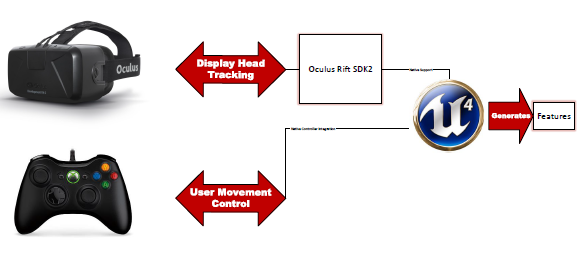
\includegraphics[scale=1.0]{Diagrams/SystemDiagram.png}
 \caption{The overall system diagram}
\end{figure}
 
 \subsection{Design Selection}
 There were a number of ways to do this project, with other graphics engines or virtual reality headsets.  The reason the Unreal Engine was chosen was because of its almost seamless integration of the Oculus Rift SDK2.  As for the Oculus Rift, that was chosen because there was an available SDK2 from Nick Newell at Echostar who graciously lent the dev kit to the design team.  
 
 \subsection{Data Structures and Algorithms}
 The Unreal Engine employs a number of data structures unique to the Engine. They each have different attributes associated with them that give them different functionality. This section will go over the objects used in this project and why they were chosen.
 
 \begin{description}
 \item[Objects] \hfill \\
 Objects are a primitive data type in the Unreal Engine.  They have basic attributes such as coordinates for positioning, as well as textures.  They are static in their position so when they are placed, they will stay put.  They are also excluded from the Blueprint system, meaning they cannot have any code associated with them.  The Objects used in the gallery consist of the paintings, walls, ceiling and floor, and any other scenery that is not interactive.
 
 \item[Actors] \hfill \\
 Actors have all of the same attributes as Objects (position, texture), however actors can be manipulated in the Blueprint system.  Their attributes can be changed for animation and signifying interactions.  In the gallery, the text-description's animation was done in the Blueprint system which was associated with each text-description actor.
 
 \item[Arrays] \hfill \\
 Arrays in the Unreal Engine behave just like in C++. They are indexed arrays and can hold any of the data types supported by the Engine (integers, booleans, strings, etc.).  The waypoint system for on-rails movement utilized an array of vectors.  Each vector was a position in the gallery, so the user could index through the array to move along in the tour.
 \end{description}
  
 \subsection{Data Flow}
  Data flow is somewhat hard to describe when using the Unreal Engine, as most of the data is global, there is little need to pass data around.  That being said, a number of the Blueprints use data associated with specific in-engine objects such as the user actor.  The user has a position vector, a vision vector, and movement vectors that all come into play in many of the Blueprints.  The vision vector is especially important because this allows the text-descriptions to play their animation only when the user is looking at them.  
 
 \subsection{Communications}
 Due to the nature of how the Oculus Rift interacts with the Unreal Engine, communication between them is handled intrinsically, the same is true for the Xbox 360 controller.  Because of this, there was little to no need for custom communication suites for this project.  The Unreal Engine automatically detects any game controller plugged in, as well as the Oculus Rift (if the correct drivers have been installed).
 
 \subsection{Classes}
 The classes used in the creation of this project are all standard to the Unreal Engine.  The classes being:
 \begin{enumerate}
 \item Actors
 \item Objects
 \end{enumerate}
 
These are described in detail above in the data structures and algorithms section.
 %\subsection{UML}
 
 %\subsection{GUI}
 
 %\subsection{MVVM, etc}

\section{ Movement }


\subsection{Technologies  Used}
\begin{enumerate}
	\item Unreal Engine Blueprint
	\item Oculus Rift
	\item Keyboard and mouse
	\item Xbox 360 wired controller
\end{enumerate}

\subsection{Component  Overview}

% SHOULD REVISE THIS SECTION
\begin{enumerate}
	\item Free movement:  User can freely move throughout the environment
	\item On-rails:  User travels from painting to painting along a linear path
\end{enumerate}

%\subsection{Phase Overview}
%This is an extension of the Phase Overview above, but specific to this component. 
% It is meant to be basically a brief list with space for marking the phase status. 

\subsection{ Architecture  Diagram}
\begin{figure}
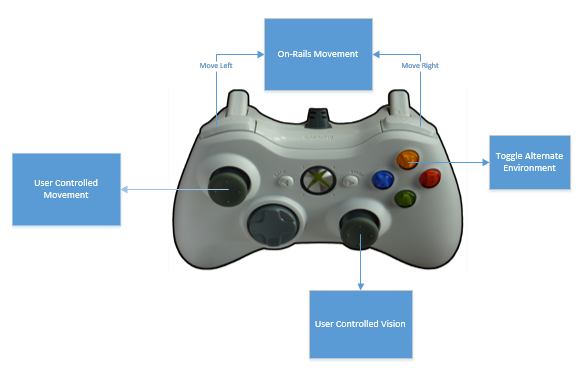
\includegraphics[scale=1.0]{Diagrams/XboxControlDiagram.png}
\centering
\caption{Movement controls for the user}
\end{figure}


%\subsection{Data Flow Diagram}
%INSERT BLUEPRINTS HERE


\subsection{Design Details}
The movement methods are a key feature to this product.  Without a good movement system, the user will not feel immersed in the gallery and will detract from the experience.  The reason for two different methods is that the design team felt that on-rails would be a better fit for users who are inexperienced with virtual reality or handheld controller input.  The free-movement will be a better fit for people who have experience with virtual reality, or who are familiar with standard movement controls for the Xbox 360.

\subsection{Blueprints}
These are the code segments that controls user movement.

\begin{figure}
\centering
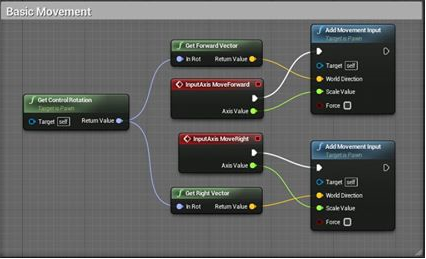
\includegraphics[scale=1.0]{Blueprints/basicMovement.png}
\caption{User controlled movement}
\end{figure}

\begin{figure}
\centering
\begin{minipage}{0.45\textwidth}
\centering
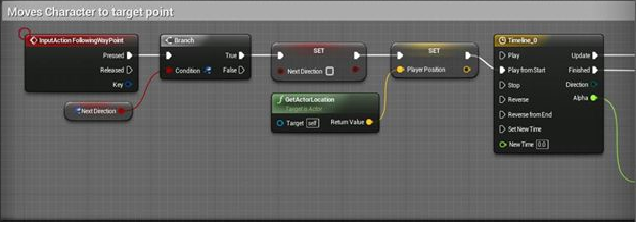
\includegraphics[scale=0.5]{Blueprints/moveToPoint.png}
\caption{First half of on-rails movement}
\end{minipage}\hfill
\begin{minipage}{0.45\textwidth}
\centering
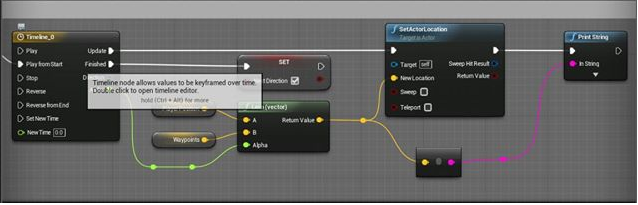
\includegraphics[scale=0.5]{Blueprints/moveToPoint2.png}
\caption{Second half of on-rails blueprint}
\end{minipage}
\end{figure}
%Should probably add more to this section



\section{Paintings }

\subsection{Technologies  Used}
\begin{enumerate}
\item Unreal Engine 4.0 Blueprint system
\end{enumerate}

\subsection{Component  Overview}
\begin{enumerate}
\item Painting image files (.png)
\item Painting texture files
\item UE objects with textures attached
\end{enumerate}

%\subsection{Phase Overview}
%I'm not exactly sure what to put for this or any of the phase overviews 


\subsection{Design Details}
The paintings were a main feature of the project, and accurately representing the artist's vision was a priority in designing.  With this in mind, the design team made sure to maximize viewing experience by increasing the size of the paintings but keeping the same scale.  This allowed users to easily view the pieces without having to walk right up to them.  There was a slight bottleneck in viewing quality when it came to seeing it with the Oculus.  Since the SDK2 had a very limited resolution, the paintings and gallery itself might appear pixelated, and sadly there was nothing to be done about that.

Creating the actual picture objects was a tedious process due to the fact that every picture file had to be converted from .jpg to .png in order for them to work in the engine.  Then was the task of making the objects in the right dimension for each painting which was done by making box objects to scale with the width and height of each painting, then dragging the .png file onto the object itself thereby creating the texture.


\section{Gallery}

\subsection{Technologies  Used}
\begin{enumerate}
\item Unreal Engine 4.0
\item Measuring Tape
\end{enumerate}


\subsection{Component  Overview}
The gallery itself was fairly easy to generate.  A blueprint of the actual room was provided by the Dahl and make rendering the Unreal Engine as simple as make the right sized objects.  The four outer walls were very easy to generate from the blueprint, the two protruding walls had to be measured by hand. The rounded corners however were more difficult to recreate because there are no rounded walls in the Unreal Engine, so they had to be custom made.  

%WHAT DO WE PUT FOR PHASE OVERVIEW
%\subsection{Phase Overview}
%This is an extension of the Phase Overview above, but specific to this component. 
% It is meant to be basically a brief list with space for marking the phase status. 

\subsection{ Architecture  Diagram}
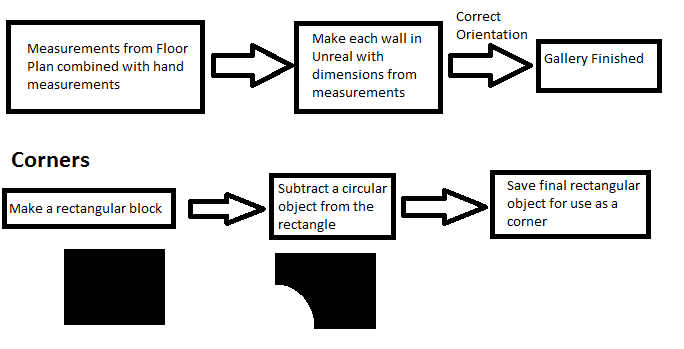
\includegraphics[scale=1.0]{Diagrams/GalleryDiagram.png}


%\subsection{Data Flow Diagram}
%INSERT BLUEPRINTS HERE



\subsection{Design Details}
This section is about how the actual room was recreated in the Unreal Engine.  The Dahl provided a blueprint of the room which gave the dimensions and angles of the corners which was helpful in mapping it into the engine.  A measuring tape was used for the standalone walls that protrude into the room and the measurements were then scaled to the Unreal Engine unit system.  As for the rounded corners, they were made using a solid block in the Engine, then subtracting a cylinder from that.

\section{Text Descriptions}

\subsection{Technologies Used}
	\begin{enumerate}
		\item Unreal Engine 4.0
	\end{enumerate}

\subsection{Component Overview}
The text descriptions as described in the user stories, are interpretive excerpts written by the artist Arthur Amiotte that give insight into the meaning behind the piece.  The way the design team implemented these descriptions in the gallery is by using small rectangular objects that expand when the user is looking at the painting, in order to provide ease of reading, and then shrink back down when the user moves on.  The actual text that will appear on this object will come from a .png file and just like the paintings, be applied to in-gallery objects. 

\subsection{Architecture Diagram}
\subsection{Data Flow Diagram}
%INSERT BLUEPRINTS HERE

\subsection{Design Details}
This component was designed very similarly to the paintings, in that the method of applying this "text-texture" to the in-gallery objects was the same.  The main difference between the two, is the enlarging and shrinking of the object.  This was done using a blueprint in the Unreal Engine Blueprint editor, the blueprint itself can be viewed above in the Data Flow Diagram section.  

\subsection{Blueprints}
\begin{figure}
\centering
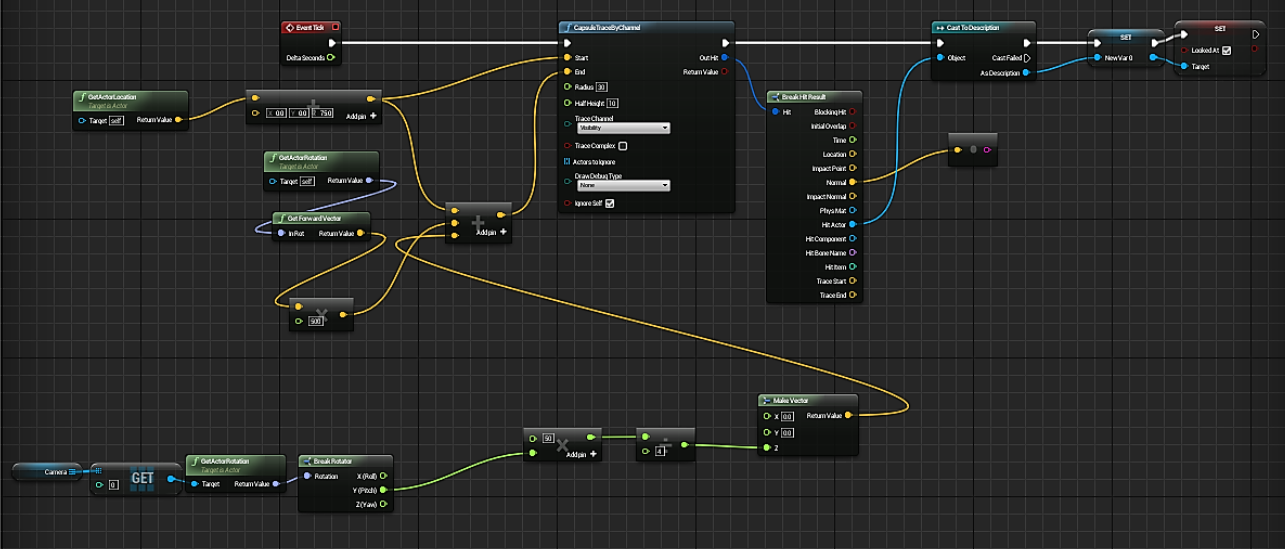
\includegraphics[scale=0.5]{Blueprints/TextDescription1.png}
\caption{The blueprint that gets the direction the user is facing}
\end{figure}
\begin{figure}
\centering
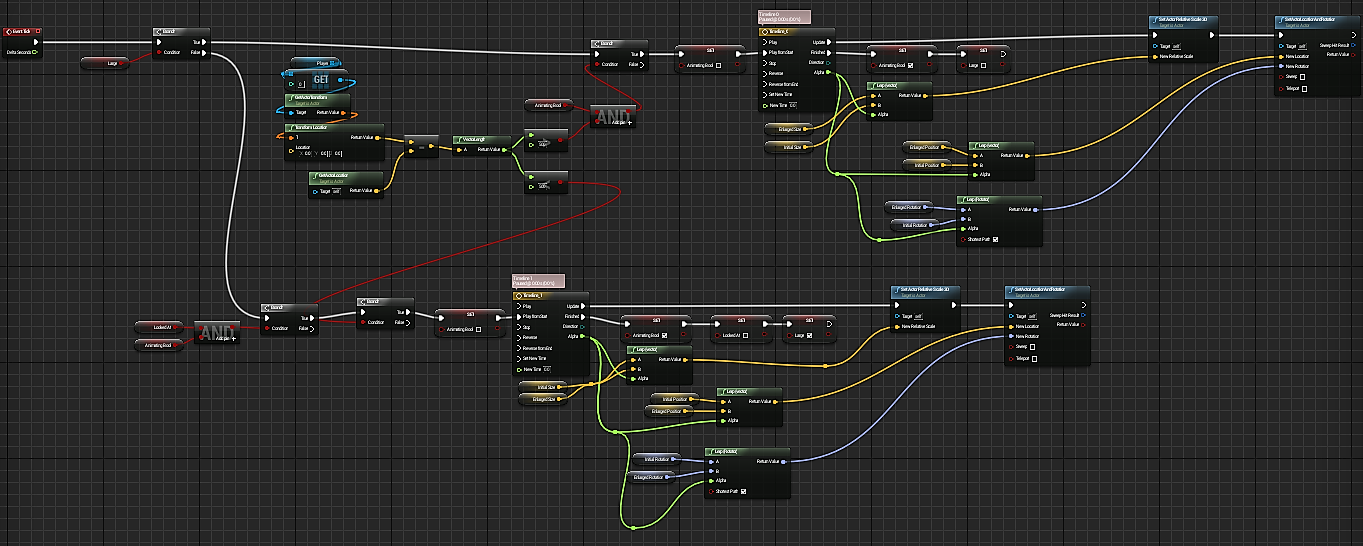
\includegraphics[scale=0.5]{Blueprints/TextDescription2.png}
\caption{Blueprint that handles the animation of the text description}
\end{figure}

\section{Alternate Environment}

\subsection{Technologies Used}
\begin{enumerate}
\item terrain.party:  height map generator
\item Unreal Engine height map integrator
\end{enumerate}

\subsection{Component Overview}
The alternate environment was added to this project in the first meeting with the Dahl Committee, after a member of the design team suggested the idea.  The Black Hills was chosen as the environment due to the significance of the artist. 
Although the static mesh of the alternate environment is actually the Black Hills, the scenery such as the trees and shrubbery is not authentic.  There are no Ponderosa Pine tree (or other native fauna) assets in the Unreal Engine, and it was out of the scope of the project to custom create them.  That being said, the scenery does not appear to detract from the experience according to the number of people who gave it a try.


\subsection{Architecture Diagram}
\begin{figure}
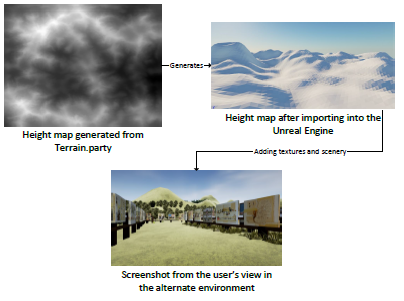
\includegraphics[scale=1.0]{Diagrams/AltEnvironment.png}
\centering
\caption{How the alternate environment was generated}
\end{figure}

\subsection{Design Details}
When the idea of the alternate environment was first brought up, the design team had a rough idea of how to go about creating it.  The original idea was to go out into the Hills and take a panoramic photograph of the horizon, then (much like the paintings and text-descriptions) apply it as a texture to a UE object.  Thankfully this awful idea was replaced once Alex discovered terrain.party.  This made it amazingly simple to generate a height map, simply by selecting a region and downloading a .zip file containing the map files.  Then, using the native height map support in the Unreal Engine, the static mesh was created and modified to accommodate the gallery recreation, replacing the walls with wooden fences.

